\section{Exercises}


%_________________
\subsection{Case study}

% 1

\eoce{\qt{Migraine and acupuncture}
A migraine is a particularly painful type of headache, which patients sometimes wish to treat with acupuncture. To determine whether acupuncture relieves migraine pain, researchers conducted a randomized controlled study where 89 females diagnosed with migraine headaches were randomly assigned to one of two groups: treatment or control. 43 patients in the treatment group received acupuncture that is specifically designed to treat migraines. 46 patients in the control group received placebo acupuncture (needle insertion at nonacupoint locations). 24 hours after patients received acupuncture, they were asked if they were pain free. Results are summarized in the contingency table below. \footfullcite{Allais:2011}

\noindent\begin{minipage}[l]{0.4\textwidth}
\begin{tabular}{ll  cc c} 
			&				& \multicolumn{2}{c}{\textit{Pain free}} \\
\cline{3-4}
			&							& Yes 	& No 	& Total	\\
\cline{2-5}
							&Treatment 	& 10	 	& 33		& 43 	\\
\raisebox{1.5ex}[0pt]{\emph{Group}}	& Control		& 2	 	& 44 	 	& 46 \\
\cline{2-5}
							&Total		& 12		& 77		& 89
\end{tabular}
\end{minipage}
\begin{minipage}[c]{0.05\textwidth}
\end{minipage}
\begin{minipage}[c]{0.27\textwidth}
\begin{center}
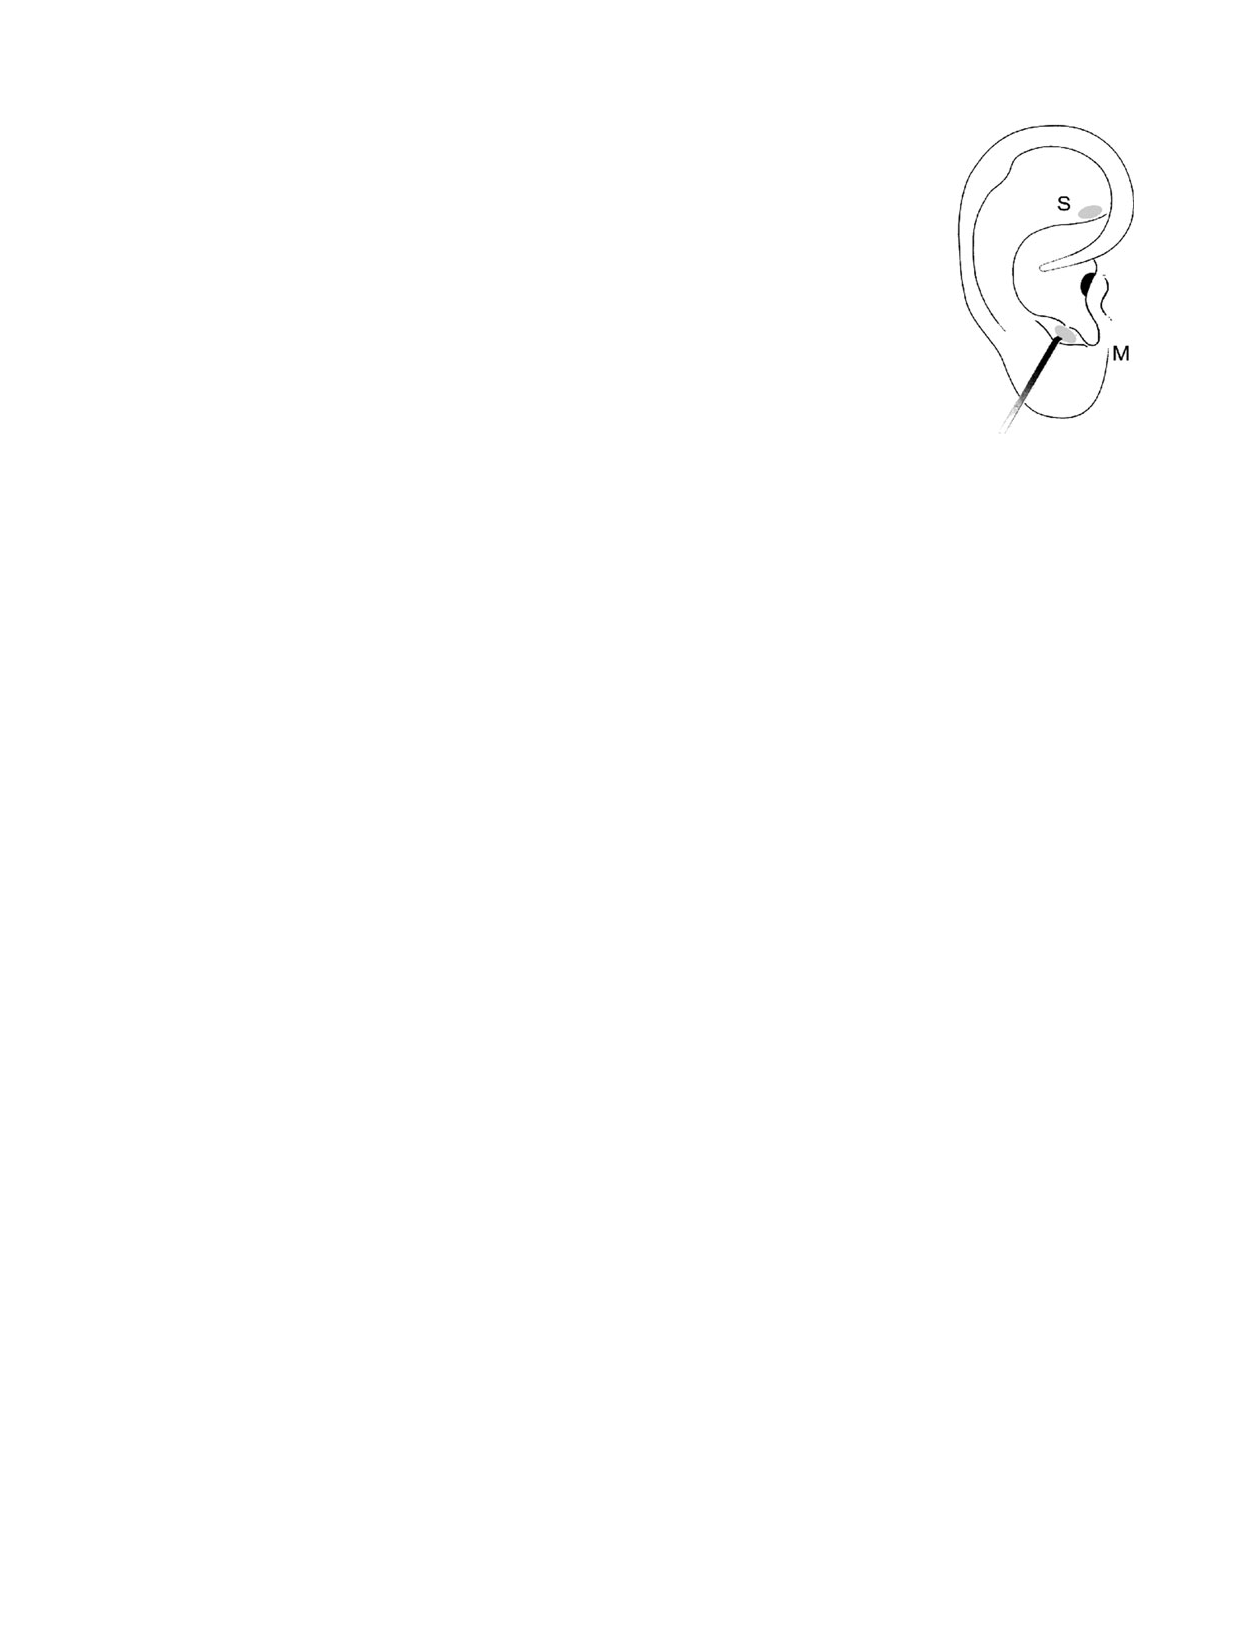
\includegraphics[width = 0.75\textwidth]{01/figures/eoce/images/earacupuncture}
\end{center}
\end{minipage}
\begin{minipage}[c]{0.25\textwidth}
{\footnotesize Figure from the original paper displaying the appropriate area (M) versus the inappropriate area (S) used in the treatment of migraine attacks.}
\end{minipage}
\begin{parts}
\item What percent of patients in the treatment group were pain free 24 hours after receiving acupuncture? What percent in the control group?
\item At first glance, does acupuncture appear to be an effective treatment for migraines? Explain your reasoning.
\item Do the data provide convincing evidence that there is a real pain reduction for those patients in the treatment group? Or do you think that the observed difference might just be due to chance?
\end{parts}
}
{}

% 2

\eoce{\qt{Sinusitis and antibiotics, Part I\label{sinusitis}} Researchers studying the effect of antibiotic treatment for acute sinusitis compared to symptomatic treatments randomly assigned 166 adults diagnosed with acute sinusitis to one of two groups: treatment or control. Study participants received either a 10-day course of amoxicillin (an antibiotic) or a placebo similar in appearance and taste. The placebo consisted of symptomatic treatments such as acetaminophen, nasal decongestants, etc. At the end of the 10-day period patients were asked if they experienced significant improvement in symptoms. The distribution of responses are summarized below. \footfullcite{Garbutt:2012}
\begin{center}
\begin{tabular}{ll  cc c} 
			&				& \multicolumn{2}{c}{\textit{Self-reported significant}} \\
			&				& \multicolumn{2}{c}{\textit{improvement in symptoms}} \\
\cline{3-4}
			&							& Yes 	& No 	& Total	\\
\cline{2-5}
							&Treatment 	& 66	 	& 19		& 85 	\\
\raisebox{1.5ex}[0pt]{\emph{Group}}	& Control		& 65	 	& 16 	 	& 81 \\
\cline{2-5}
							&Total		& 131	& 35		& 166
\end{tabular}
\end{center}
\begin{parts}
\item What percent of patients in the treatment group experienced a significant improvement in symptoms? What percent in the control group?
\item Based on your findings in part (a), which treatment appears to be more effective for sinusitis?
\item Do the data provide convincing evidence that there is a difference in the improvement rates of sinusitis symptoms? Or do you think that the observed difference might just be due to chance?
\end{parts}
}
{}


%_________________
\subsection{Data basics}

% 3

\eoce{\qt{Identify study components, Part I\label{components1}} Identify (i) the cases, (ii) the variables and their types, and (iii) the main research question in the studies described below.
\begin{parts}
\item Researchers collected data to examine the relationship between pollutants and preterm births in Southern California. During the study air pollution levels were measured by air quality monitoring stations. Specifically, levels of carbon monoxide were recorded in parts per million, nitrogen dioxide and ozone in parts per hundred million, and coarse particulate matter (PM$_{10}$) in $\mu g/m^3$. Length of gestation data were collected on 143,196 births between the years 1989 and 1993, and air pollution exposure during gestation was calculated for each birth. The analysis suggested that increased ambient PM$_{10}$ and, to a lesser degree, CO concentrations may be associated with the occurrence of preterm births. \footfullcite{Ritz+Yu+Chapa+Fruin:2000}
\item The Buteyko method is a shallow breathing technique developed by Konstantin Buteyko, a Russian doctor, in 1952. Anecdotal evidence suggests that the Buteyko method can reduce asthma symptoms and improve quality of life. In a scientific study to determine the effectiveness of this method, researchers recruited 600 asthma patients aged 18-69 who relied on medication for asthma treatment. These patients were split into two research groups: one practiced the Buteyko method and the other did not. Patients were scored on quality of life, activity, asthma symptoms, and medication reduction on a scale from 0 to 10. On average, the participants in the Buteyko group experienced a significant reduction in asthma symptoms and an improvement in quality of life. \footfullcite{McDowan:2003}
\end{parts}
}{}

% 4

\eoce{\qt{Identify study components, Part II\label{components2}} Identify (i) the cases, (ii) the variables and their types, and (iii) the main research question of the studies described below.
\begin{parts}
\item While obesity is measured based on body fat percentage (more than 35\% body fat for women and more than 25\% for men), precisely measuring body fat percentage is difficult. Body mass index (BMI), calculated as the ratio $weight/height^2$, is often used as an alternative indicator for obesity. A common criticism of BMI is that it assumes the same relative body fat percentage regardless of age, sex, or ethnicity. In order to determine how useful BMI is for predicting body fat percentage across age, sex and ethnic groups, researchers studied 202 black and 504 white adults who resided in or near New York City, were ages 20-94 years old, had BMIs of 18-35 kg/m$^2$, and who volunteered to be a part of the study. Participants reported their age, sex, and ethnicity and were measured for weight and height. Body fat percentage was measured by submerging the participants in water. \footfullcite{Gallagher:1996} \label{BMIAgeSexEth}

\item In a study of the relationship between socio-economic class and unethical behavior, 129 University of California undergraduates at Berkeley were asked to identify themselves as having low or high social-class by comparing themselves to others with the most (least) money, most (least) education, and most (least) respected jobs. They were also presented  with a jar of individually wrapped candies and informed that they were for children in a nearby laboratory, but that they could take some if they wanted. Participants completed unrelated tasks and then reported the number of candies they had taken. It was found that those in the upper-class rank condition took more candy than did those in the lower-rank condition. \footfullcite{Piff:2012}
\end{parts}
}{}

% 5
\textB{\pagebreak}

\eoce{\qt{Fisher's irises} Sir Ronald Aylmer Fisher was an English statistician, evolutionary biologist, and geneticist who worked on a data set that contained sepal length and width, and petal length and width from three species of iris flowers (\textit{setosa}, \textit{versicolor} and \textit{virginica}). There were 50 flowers from each species in the data set. \footfullcite{Fisher:1936,irisPic} \\
\noindent\begin{minipage}[c]{0.55\textwidth}
\begin{parts}
\item How many cases were included in the data?
\item How many numerical variables are included in the data? Indicate what they are, and if they are continuous or discrete.
\item How many categorical variables are included in the data, and what are they? List the corresponding levels (categories).
\end{parts} \vspaceB{10mm}
\end{minipage}
\begin{minipage}[c]{0.4\textwidth}
\begin{center}
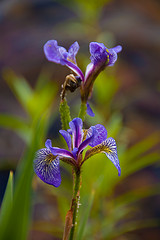
\includegraphics[width = 30mm]{01/figures/eoce/images/irisversicolor}
\end{center}
\end{minipage}
}{}

% 6

\eoce{\qt{Smoking habits of UK residents\label{UKSmoking_datamatrix}} A survey was conducted to study the smoking habits of UK residents. Below is a data matrix displaying a portion of the data collected in this survey. Note that ``$\pounds$" stands for British Pounds Sterling, ``cig" stands for cigarettes, and ``N/A'' refers to a missing component of the data. \footfullcite{data:smoking}
\begin{table}[h]
\begin{center}
\scriptsize{
\begin{tabular}{rccccccc}
  \hline
 & gender & age & marital & grossIncome & smoke & amtWeekends & amtWeekdays \\ 
  \hline
1 & Female &  42 & Single & Under $\pounds$2,600 & Yes &  12 cig/day &  12 cig/day \\ 
2 & Male &  44 & Single & $\pounds$10,400 to $\pounds$15,600 & No & N/A & N/A \\ 
3 & Male &  53 & Married & Above $\pounds$36,400 & Yes &   6 cig/day &   6 cig/day \\ 
\vdots & \vdots &  \vdots & \vdots & \vdots & \vdots & \vdots & \vdots \\ 
1691 & Male &  40 & Single & $\pounds$2,600 to $\pounds$5,200 & Yes &   8 cig/day &   8 cig/day \\   
   \hline
\end{tabular}
}
\end{center}
\end{table}
\begin{parts}
\item What does each row of the data matrix represent?
\item How many participants were included in the survey?
\item Indicate whether each variable in the study is numerical or categorical. If numerical, identify as continuous or discrete. If categorical, indicate if the variable is ordinal.
\end{parts}
}{}


%_________________
\subsection{Overview of data collection principles}

% 7

\eoce{\qt{Generalizability and causality, Part I} Identify the population of interest and the sample in the studies described in Exercise~\ref{components1}. Also comment on whether or not the results of the study can be generalized to the population and if the findings of the study can be used to establish causal relationships.
}{}

% 8

\eoce{\qt{Generalizability and causality, Part II} Identify the population of interest and the sample in the studies described in Exercise~\ref{components2}. Also comment on whether or not the results of the study can be generalized to the population and if the findings of the study can be used to establish causal relationships.
}{}

% 9
\textB{\pagebreak}

\eoce{\qt{GPA and study time} A survey was conducted on 218 undergraduates from Duke University who took an introductory statistics course in Spring 2012. Among many other questions, this survey asked them about their GPA and the number of hours they spent studying per week. The scatterplot below displays the relationship between these two variables.

\noindent\begin{minipage}[c]{0.44\textwidth}
\begin{parts}
\item What is the explanatory variable and what is the response variable?
\item Describe the relationship between the two variables. Make sure to discuss unusual observations, if any.
\item Is this an experiment or an observational study?
\item Can we conclude that studying longer hours leads to higher GPAs?
\end{parts} \vspaceB{4mm}
\end{minipage}
\begin{minipage}[c]{0.55\textwidth}
\begin{center}
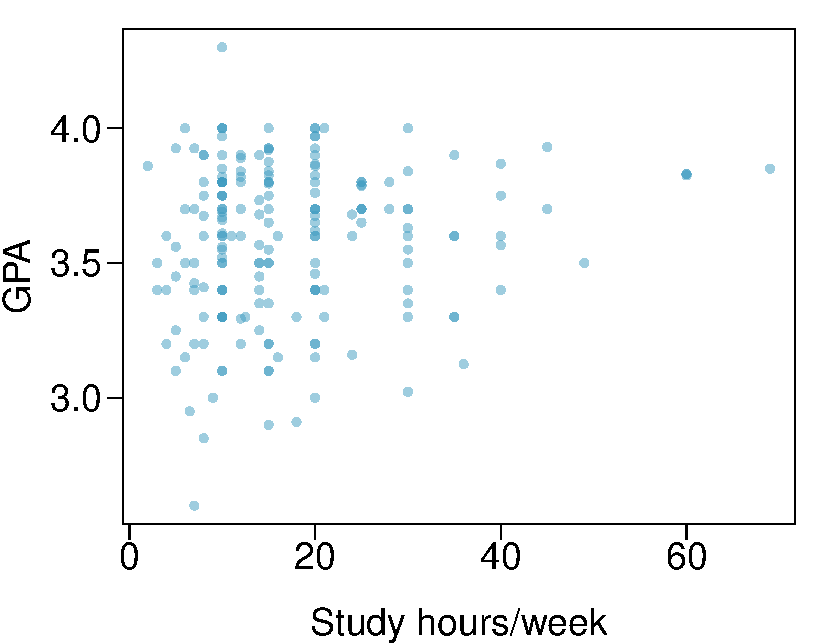
\includegraphics[width = 0.88\textwidth]{01/figures/eoce/gpaStudy/gpaStudy}
\end{center}
\end{minipage}
}{}


% 10

\eoce{\qt{Income and education} The scatterplot below shows the relationship between per capita income (in thousands of dollars) and percent of population with a bachelor's degree in 3,143 counties in the US in 2010.

\noindent\begin{minipage}[c]{0.44\textwidth}
\begin{parts}
\item What are the explanatory and response variables?
\item Describe the relationship between the two variables. Make sure to discuss unusual observations, if any.
\item Can we conclude that having a bachelor's degree increases one's income?
\end{parts} \vspaceB{16mm}
\end{minipage}
\begin{minipage}[c]{0.55\textwidth}
\begin{center}
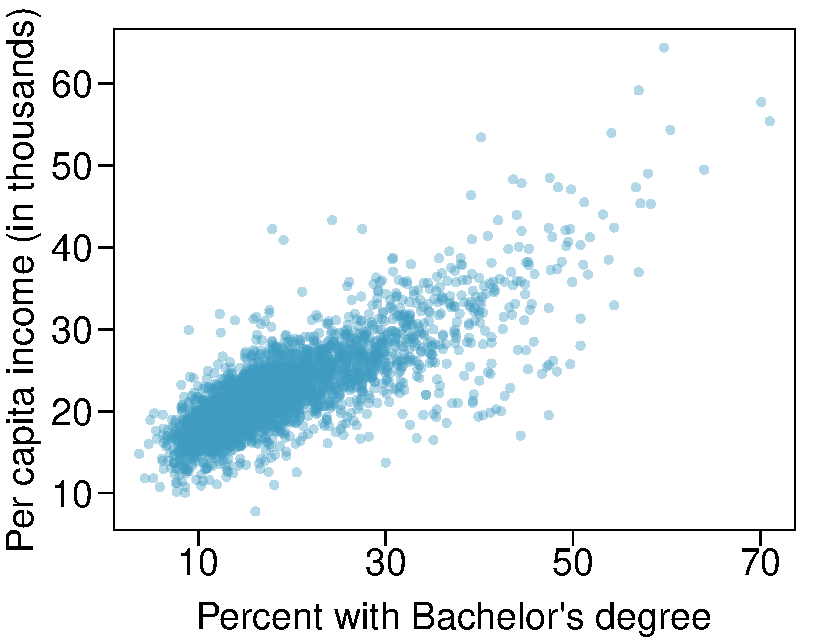
\includegraphics[width = 0.88\textwidth]{01/figures/eoce/county/county_incomeBach}
\end{center}
\end{minipage}
}{}


%_________________
\subsection{Observational studies and sampling strategies}

% 11

\eoce{\qt{Propose a sampling strategy} A large college class has 160 students. All 160 students attend the lectures together, but the students are divided into 4 groups, each of 40 students, for lab sections administered by different teaching assistants. The professor wants to conduct a survey about how satisfied the students are with the course, and he believes that the lab section a student is in might affect the student's overall satisfaction with the course.
\begin{parts}
\item What type of study is this?
\item Suggest a sampling strategy for carrying out this study.
\end{parts}
}{}


% 12
\textB{\pagebreak}

\eoce{\qt{Internet use and life expectancy} The scatterplot below shows the relationship between estimated life expectancy at birth as of 2012\footfullcite{data:ciaFactBookLifeExp:2012} and percentage of internet users in 2010\footfullcite{data:ITU:2012} in 208 countries.

\noindent\begin{minipage}[c]{0.43\textwidth}
\begin{parts}
\item Describe the relationship between life expectancy and percentage of internet users.
\item What type of study is this?
\item State a possible confounding variable that might explain this relationship and describe its potential effect.
\end{parts}\vspace{16mm}
\end{minipage}%
\begin{minipage}[r]{0.55\textwidth}
\hfill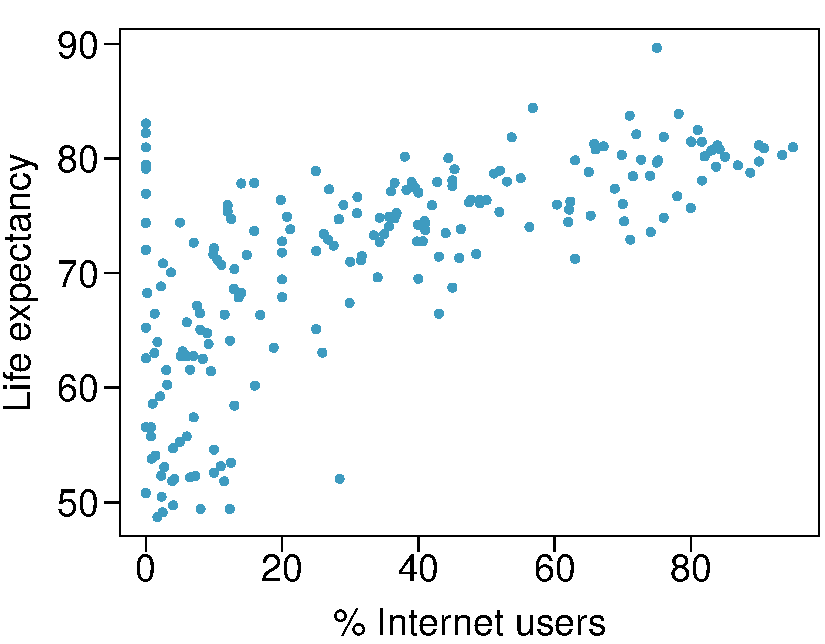
\includegraphics[width = 0.95\textwidth]{01/figures/eoce/country/county_lifeExpInter}
\end{minipage}
}{}

% 13

\eoce{\qt{Random digit dialing} The Gallup Poll uses a procedure called random digit dialing, which creates phone numbers based on a list of all area codes in America in conjunction with the associated number of residential households in each area code. Give a possible reason the Gallup Poll chooses to use random digit dialing instead of picking phone numbers from the phone book.
}{}

% 14

\eoce{\qt{Sampling strategies} A statistics student who is curious about the relationship between the amount of time students spend on social networking sites and their performance at school decides to conduct a survey. Three research strategies for collecting data are described below. In each, name the sampling method proposed and any bias you might expect.
\begin{parts}
\item He randomly samples 40 students from the study's population, gives them the survey, asks them to fill it out and bring it back the next day.
\item He gives out the survey only to his friends, and makes sure each one of them fills out the survey.
\item He posts a link to an online survey on his Facebook wall and asks his friends to fill out the survey.
\APVersion{\item He stands outside the student center and asks every third person that walks out the door to fill out the survey.}
\end{parts}
}{}


% 15

\eoce{\qt{Family size} Suppose we want to estimate family size, where family is defined as one or more parents living with children. If we select students at random at an elementary school and ask them what their family size is, will our average be biased? If so, will it overestimate or underestimate the true value?
}{}


\textB{\newpage}

% 16

\eoce{\qt{Flawed reasoning} Identify the flaw in reasoning in the following scenarios. Explain what the individuals in the study should have done differently if they wanted to make such strong conclusions.
\begin{parts}
\item Students at an elementary school are given a questionnaire that they are required to return after their parents have completed it. One of the questions asked is, ``Do you find that your work schedule makes it difficult for you to spend time with your kids after school?" Of the parents who replied, 85\% said ``no". Based on these results, the school officials conclude that a great majority of the parents have no difficulty spending time with their kids after school.
\item A survey is conducted on a simple random sample of 1,000 women who recently gave birth, asking them about whether or not they smoked during pregnancy. A follow-up survey asking if the children have respiratory problems is conducted 3 years later, however, only 567 of these women are reached at the same address. The researcher reports that these 567 women are representative of all mothers.
\item A orthopedist administers a questionnaire to 30 of his patients who do not have any joint problems and finds that 20 of them regularly go running. He concludes that running decreases the risk of joint problems.
\end{parts}
}{}


% 17

\eoce{\qt{Reading the paper} Below are excerpts from two articles published in the \emph{NY Times}:
\begin{parts}
\item An article called \emph{Risks: Smokers Found More Prone to Dementia} states the following: \footfullcite{news:smokingDementia}
\begin{adjustwidth}{2em}{2em}
{\footnotesize ``Researchers analyzed the data of 23,123 health plan members who participated in a voluntary exam and health behavior survey from 1978 to 1985, when they were 50 to 60 years old. Twenty-three years later, about one-quarter of the group, or 5,367, had dementia, including 1,136 with Alzheimer�s disease and 416 with vascular dementia. After adjusting for other factors, the researchers concluded that pack-a-day smokers were 37 percent more likely than nonsmokers to develop dementia, and the risks went up sharply with increased smoking; 44 percent for one to two packs a day; and twice the risk for more than two packs."}
\end{adjustwidth}
Based on this study, can we conclude that smoking causes dementia later in life? Explain your reasoning.
\item Another article called \emph{The School Bully Is Sleepy} states the following: \footfullcite{news:bullySleep}
\begin{adjustwidth}{2em}{2em}
{\footnotesize ``The University of Michigan study, collected survey data from parents on each child's sleep habits and asked both parents and teachers to assess behavioral concerns. About a third of the students studied were identified by parents or teachers as having problems with disruptive behavior or bullying. The researchers found that children who had behavioral issues and those who were identified as bullies were twice as likely to have shown symptoms of sleep disorders."}
\end{adjustwidth}
A friend of yours who read the article says, ``The study shows that sleep disorders lead to bullying in school children." Is this statement justified? If not, how best can you describe the conclusion that can be drawn from this study?
\end{parts}
}{}


% 18

\eoce{\qt{Shyness on Facebook} Given the anonymity afforded to individuals in online interactions, researchers hypothesized that shy individuals would have more favorable attitudes toward Facebook and that shyness would be positively correlated with time spent on Facebook. They also hypothesized that shy individuals would have fewer Facebook ``Friends" just like they have fewer friends than non-shy individuals have in the offline world. Data were collected on 103 undergraduate students at a university in southwestern Ontario via online questionnaires. The study states ``Participants were recruited through the university's psychology participation pool. After indicating an interest in the
study, participants were sent an e-mail containing the study's URL as well as the necessary login credentials." Are the results of this study generalizable to the population of all Facebook users? \footfullcite{Orr:2009}
}{}


%_________________
\textB{\pagebreak}
\subsection{Experiments}

% 19

\eoce{\qt{Vitamin supplements} In order to assess the effectiveness of taking large doses of vitamin C in reducing the duration of the common cold, researchers recruited 400 healthy volunteers from staff and students at a university. A quarter of the patients were assigned a placebo, and the rest were evenly divided between 1g Vitamin C,  3g Vitamin C, or 3g Vitamin C plus additives to be taken at onset of a cold for the following two days. All tablets had identical appearance and packaging. The nurses who handed the prescribed pills to the patients knew which patient received which treatment, but the researchers assessing the patients when they were sick did not. No significant differences were observed in any measure of cold duration or severity between the four medication groups, and the placebo group had the shortest duration of symptoms.\footfullcite{Audera:2001}
\begin{parts}
\item Was this an experiment or an observational study? Why?
\item What are the explanatory and response variables in this study?
\item Were the patients blinded to their treatment?
\item Was this study double-blind?
\item Participants are ultimately able to choose whether or not to use the pills prescribed to them. We might expect that not all of them will adhere and take their pills. Does this introduce a confounding variable to the study? Explain your reasoning.
\end{parts}
}{}


% 20

\eoce{\qt{Soda preference} You would like to conduct an experiment in class to see if your classmates prefer the taste of regular Coke or Diet Coke. Briefly outline a design for this study.
}{}


% 21

\eoce{\qt{Exercise and mental health} A researcher is interested in the effects of exercise on mental health and he proposes the following study: Use stratified random sampling to ensure representative proportions of 18-30, 31-40 and 41-55 year olds from the population. Next, randomly assign half the subjects from each age group to exercise twice a week, and instruct the rest not to exercise. Conduct a mental health exam at the beginning and at the end of the study, and compare the results.
\begin{parts}
\item What type of study is this? 
\item What are the treatment and control groups in this study?
\item Does this study make use of blocking? If so, what is the blocking variable?
\item Does this study make use of blinding?
\item Comment on whether or not the results of the study can be used to establish a causal relationship between exercise and mental health, and indicate whether or not the conclusions can be generalized to the population at large.
\item Suppose you are given the task of determining if this proposed study should get funding. Would you have any reservations about the study proposal?
\end{parts}
}{}


% 22
\textB{\newpage}

\eoce{\qt{Chia seeds and weight loss} Chia Pets -- those terra-cotta figurines that sprout fuzzy green hair -- made the chia plant a household name. But chia has gained an entirely new reputation as a diet supplement.  In one 2009 study, a team of researchers recruited 38 men and divided them evenly into two groups: treatment or control. They also recruited 38 women, and they randomly placed half of these participants into the treatment group and the other half into the control group. One group was given 25 grams of chia seeds twice a day, and the other was given a placebo. The subjects volunteered to be a part of the study. After 12 weeks, the scientists found no significant difference between the groups in appetite or weight loss. \footfullcite{Nieman:2009}
\begin{parts}
\item What type of study is this? 
\item What are the experimental and control treatments in this study?
\item Has blocking been used in this study? If so, what is the blocking variable?
\item Has blinding been used in this study?
\item Comment on whether or not we can make a causal statement, and indicate whether or not we can generalize the conclusion to the population at large.
\end{parts}
}{}


%_________________
\subsection{Examining numerical data}

% 23

\eoce{\qt{Mammal life spans} Data were collected on life spans (in years) and gestation lengths (in days) for 62 mammals. A scatterplot of life span versus length of gestation is shown below. \footfullcite{Allison+Cicchetti:1975}

\noindent\begin{minipage}[c]{0.5\textwidth}
\begin{parts}
\item What type of an association is apparent between life span and length of gestation?
\item What type of an association would you expect to see if the axes of the plot were reversed, i.e. if we plotted length of gestation versus life span?
\item Are life span and length of gestation independent? Explain your reasoning.
\end{parts} \vspace{9mm}
\end{minipage}
\begin{minipage}[c]{0.5\textwidth}
\begin{center}
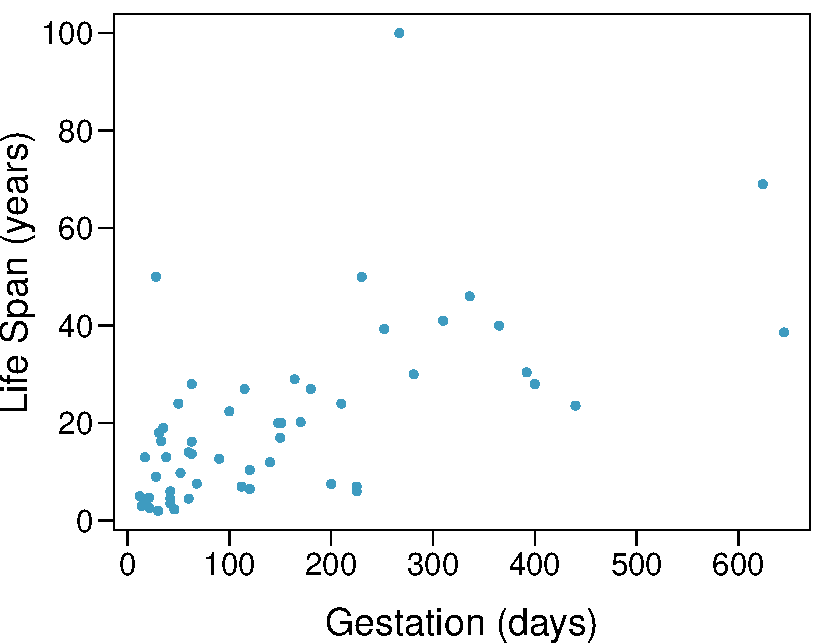
\includegraphics[width = 60mm]{01/figures/eoce/mammals/mammals_lifeSpanGest}
\end{center}
\end{minipage}
}{}


% 24

\eoce{\qt{Office productivity} Office productivity is relatively low when the employees feel no stress about their work or job security. However, high levels of stress can also lead to reduced employee productivity. Sketch a plot to represent the relationship between stress and productivity.
}{}


% 25
\textB{\newpage}

\eoce{\qt{Associations} Indicate which of the plots show a \\[1mm]
\noindent\begin{minipage}[b]{0.35\textwidth}
\begin{parts}
\item positive association
\item negative association
\item no association
\end{parts}
Also determine if the positive and negative associations are linear or nonlinear. Each part may refer to more than one plot. \vspace{31mm}
\end{minipage}%
\begin{minipage}[b]{0.62\textwidth}
\hfill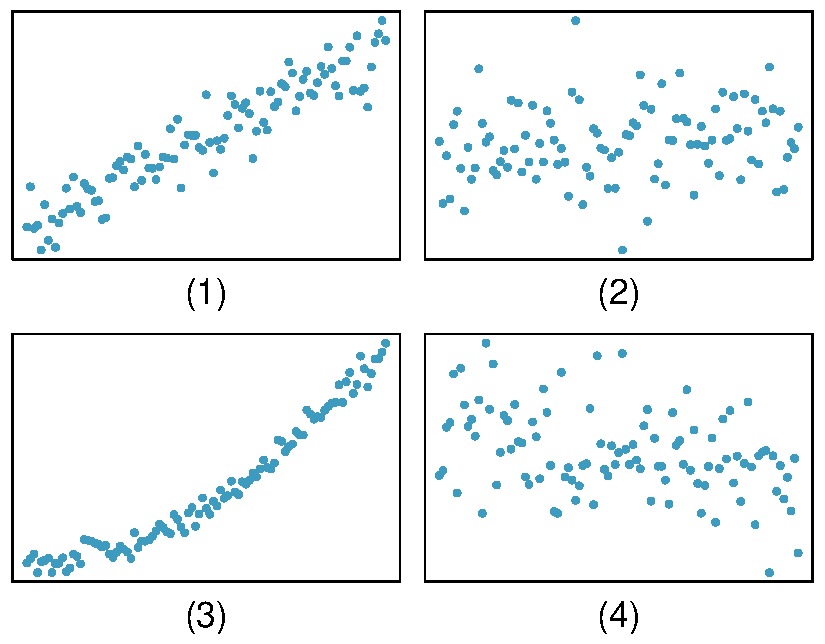
\includegraphics[width = 0.95\textwidth]{01/figures/eoce/associationPlots/associationPlots}
\end{minipage}
}{}



% 26

\eoce{\qt{Parameters and statistics} Identify which value represents the sample mean and which value represents the claimed population mean.
\begin{parts}
\item A recent article in a college newspaper stated that college students get an average of 5.5 hrs of sleep each night. A student who was skeptical about this value decided to conduct a survey by randomly sampling 25 students. On average, the sampled students slept 6.25 hours per night.
\item American households spent an average of about \$52 in 2007 on Halloween merchandise such as costumes, decorations and candy. To see if this number had changed, researchers conducted a new survey in 2008 before industry numbers were reported. The survey included 1,500 households and found that average Halloween spending was \$58 per household.
\item The average GPA of students in 2001 at a private university was 3.37. A survey on a sample of 203 students from this university yielded an average GPA of 3.59 in Spring semester of 2012.
\end{parts}
}{}


% 27

\eoce{\qt{Make-up exam} In a class of 25 students, 24 of them took an exam in class and 1 student took a make-up exam the following day. The professor graded the first batch of 24 exams and found an average score of 74 points with a standard deviation of 8.9 points. The student who took the make-up the following day scored 64 points on the exam.
\begin{parts}
\item Does the new student's score increase or decrease the average score?
\item What is the new average?
\item Does the new student's score increase or decrease the standard deviation of the scores?
\end{parts}
}{}


% 28

\eoce{\qt{Days off at a mining plant} Workers at a particular mining site receive an average of 35 days paid vacation, which is lower than the national average. The manager of this plant is under pressure from a local union to increase the amount of paid time off. However, he does not want to give more days off to the workers because that would be costly. Instead he decides he should fire 10 employees in such a way as to raise the average number of days off that are reported by his employees. In order to achieve this goal, should he fire employees who have the most number of days off, least number of days off, or those who have about the average number of days off?
}{}


% 29
\textB{\newpage}

\eoce{\qt{Smoking habits of UK residents, Part I\label{UKSmoking_amounts}} Exercise~\ref{UKSmoking_datamatrix} introduces a data set on the smoking habits of UK residents. Below are histograms displaying the distributions of the number of cigarettes smoked on weekdays and weekends, excluding non-smokers. Describe the two distributions and compare them.
\begin{center}
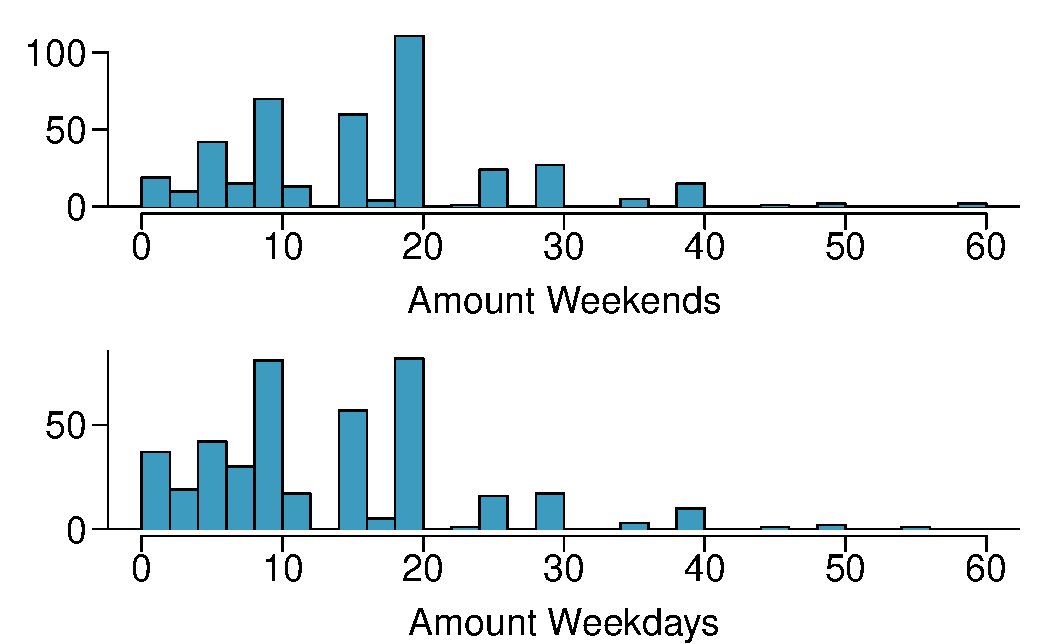
\includegraphics[width = 0.7\textwidth]{01/figures/eoce/smoking/smoking_amountHist}
\end{center}
}{}


% 30

\eoce{\qt{Stats scores\label{introStatsFinalScores}} Below are the final scores of 20 introductory statistics students.
\begin{center}
79, 83, 57, 82, 94, 83, 72, 74, 73, 71, \\
66, 89, 78, 81, 78, 81, 88, 69, 77, 79
\end{center}
Draw a histogram of these data and describe the distribution.
}{}


% 31

\eoce{\qt{Smoking habits of UK residents, Part II} A random sample of 5 smokers from the data set discussed in Exercises~\ref{UKSmoking_datamatrix} and \ref{UKSmoking_amounts} is provided below.
{\footnotesize
\begin{center}
\begin{tabular}{ccccccc}
  \hline
gender & age & maritalStatus & grossIncome & smoke & amtWeekends & amtWeekdays \\ 
  \hline
Female &  51 & Married & $\pounds$2,600 to $\pounds$5,200 & Yes &  20 cig/day &  20 cig/day\\ 
  Male &  24 & Single & $\pounds$10,400 to $\pounds$15,600 & Yes &  20 cig/day&  15 cig/day\\ 
  Female &  33 & Married & $\pounds$10,400 to $\pounds$15,600 & Yes &  20 cig/day&  10 cig/day\\ 
  Female &  17 & Single & $\pounds$5,200 to $\pounds$10,400 & Yes &  20 cig/day&  15 cig/day\\ 
  Female &  76 & Widowed & $\pounds$5,200 to $\pounds$10,400 & Yes &  20 cig/day&  20 cig/day\\ 
   \hline
\end{tabular}
\end{center}
}
\begin{parts}
\item Find the mean amount of cigarettes smoked on weekdays and weekends by these 5 respondents.
\item Find the standard deviation of the amount of cigarettes smoked on weekdays and on weekends by these 5 respondents. Is the variability higher on weekends or on weekdays?
\end{parts}
}{}


% 32

\eoce{\qt{Factory defective rate} A factory quality control manager decides to investigate the percentage of defective items produced each day. Within a given work week (Monday through Friday) the percentage of defective items produced was 2\%, 1.4\%, 4\%, 3\%, 2.2\%.
\begin{parts}
\item Calculate the mean for these data.
\item Calculate the standard deviation for these data, showing each step in detail.
\end{parts}
}{}


% 33

\eoce{\qt{Medians and IQRs} For each part, compare distributions (1) and (2) based on their medians and IQRs. You do not need to calculate these statistics; simply state how the medians and IQRs compare. Make sure to explain your reasoning. 
\begin{multicols}{2}
\begin{parts}
\item (1) 3, 5, 6, 7, 9 \\
(2) 3, 5, 6, 7, 20
\item (1) 3, 5, 6, 7, 9 \\
(2) 3, 5, 8, 7, 9
\item (1) 1, 2, 3, 4, 5 \\
(2) 6, 7, 8, 9, 10
\item (1) 0, 10, 50, 60, 100 \\
(2) 0, 100, 500, 600, 1000
\end{parts}
\end{multicols}
}{}


% 34

\eoce{\qt{Means and SDs} For each part, compare distributions (1) and (2) based on their means and standard deviations. You do not need to calculate these statistics; simply state how the means and the standard deviations compare. Make sure to explain your reasoning. \textit{Hint:} It may be useful to sketch dot plots of the distributions.
\begin{multicols}{2}
\begin{parts}
\item (1) 3, 5, 5, 5, 8, 11, 11, 11, 13 \\
(2) 3, 5, 5, 5, 8, 11, 11, 11, 20 \\
\item (1) -20, 0, 0, 0, 15, 25, 30, 30 \\
(2) -40, 0, 0, 0, 15, 25, 30, 30
\item (1) 0, 2, 4, 6, 8, 10 \\
(2) 20, 22, 24, 26, 28, 30
\item (1) 100, 200, 300, 400, 500 \\
(2) 0, 50, 300, 550, 600
\end{parts}
\end{multicols}
}{}


% 35

\eoce{\qt{Box plot} Create a box plot for the data given in Exercise~\ref{introStatsFinalScores}. The five number summary provided below may be useful.
\begin{center}
\renewcommand\arraystretch{1.5}
\begin{tabular}{ccccc}
Min	& Q1	& Q2 (Median)	& Q3	& Max \\
\hline
57	& 72.5	& 78.5	& 82.5	& 94 \\
\end{tabular}
\end{center}
}{}


% 36

\eoce{\qt{Infant mortality} The infant mortality rate is defined as the number of infant deaths per 1,000 live births. This rate is often used as an indicator of the level of health in a country. The relative frequency histogram below shows the distribution of estimated infant death rates in 2012 for 222 countries. \footfullcite{data:ciaFactBookInfMort:2012}

\noindent\begin{minipage}[c]{0.43\textwidth}
\begin{parts}
\item Estimate Q1, the median, and Q3 from the histogram.
\item Would you expect the mean of this data set to be smaller or larger than the median? Explain your reasoning.
\end{parts}
\vspace{18mm}
\end{minipage}
\begin{minipage}[c]{0.52\textwidth}
\hfill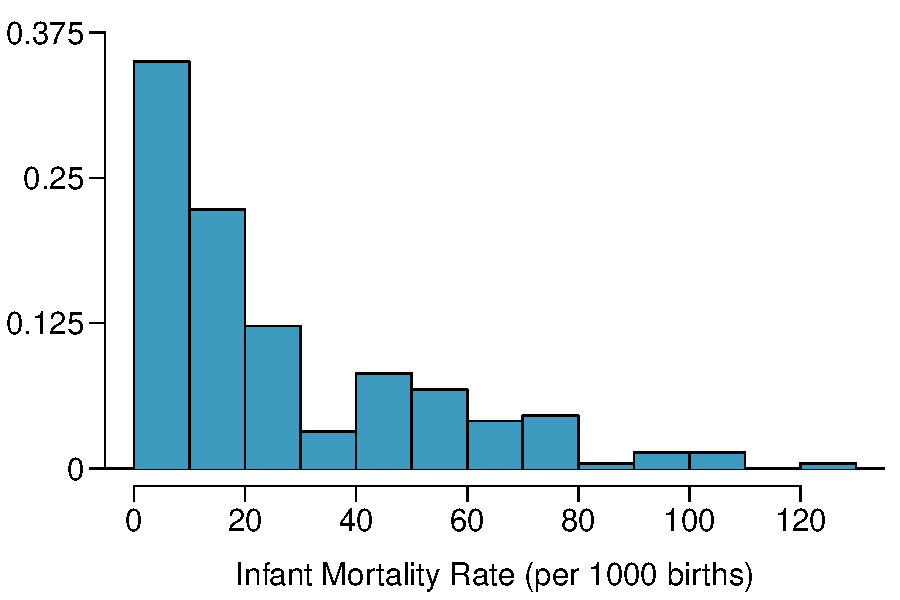
\includegraphics[width = 0.95\textwidth]{01/figures/eoce/country/country_infMort}
\end{minipage}
}{}


% 37

\eoce{\qt{Matching histograms and box plots} Describe the distribution in the histograms below and match them to the box plots. \\
\begin{center}
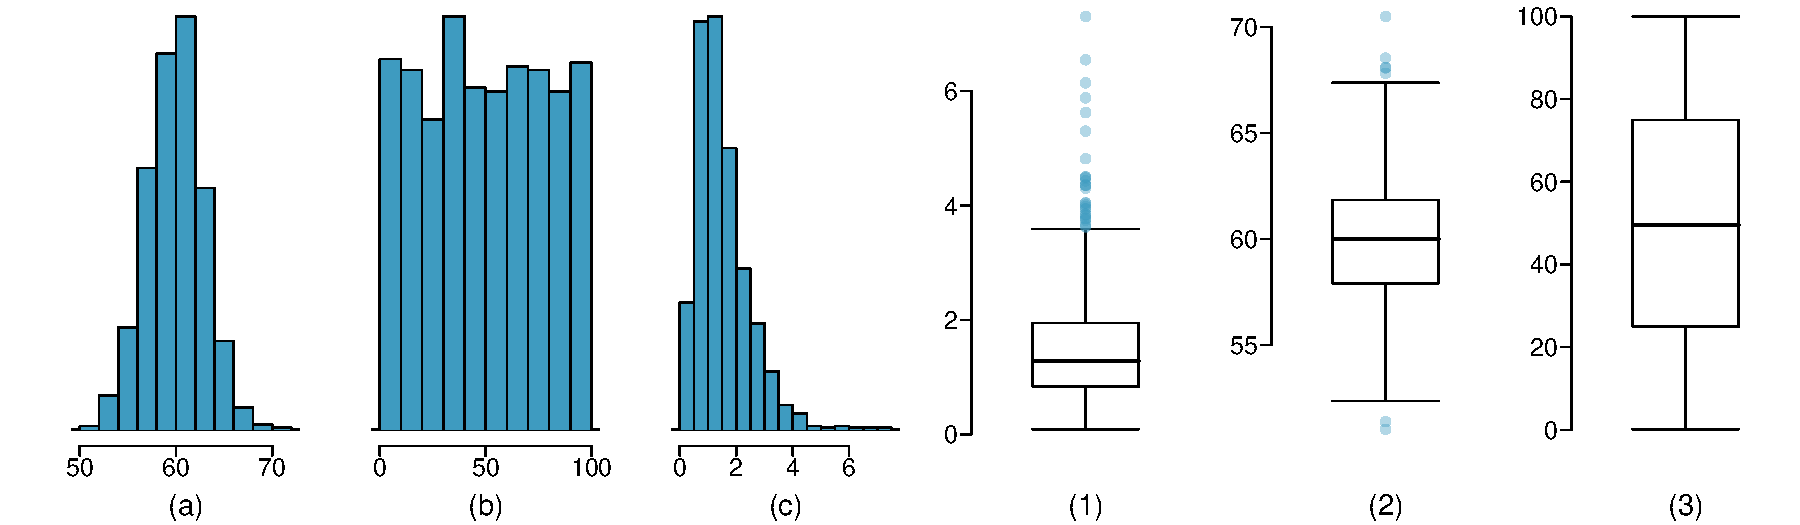
\includegraphics[width =\textwidth]{01/figures/eoce/histBoxMatch/histBoxMatch}
\end{center}
}{}


% 38
\textB{\pagebreak}

\eoce{\qt{Air quality\label{durhamAQI}} Daily air quality is measured by the air quality index (AQI) reported by the Environmental Protection Agency. This index reports the pollution level and what associated health effects might be a concern. The index is calculated for five major air pollutants regulated by the Clean Air Act. and takes values from 0 to 300, where a higher value indicates lower air quality. AQI was reported for a sample of 91 days in 2011 in Durham, NC. The relative frequency histogram below shows the distribution of the AQI values on these days. \footfullcite{data:durhamAQI:2011}
\begin{center}
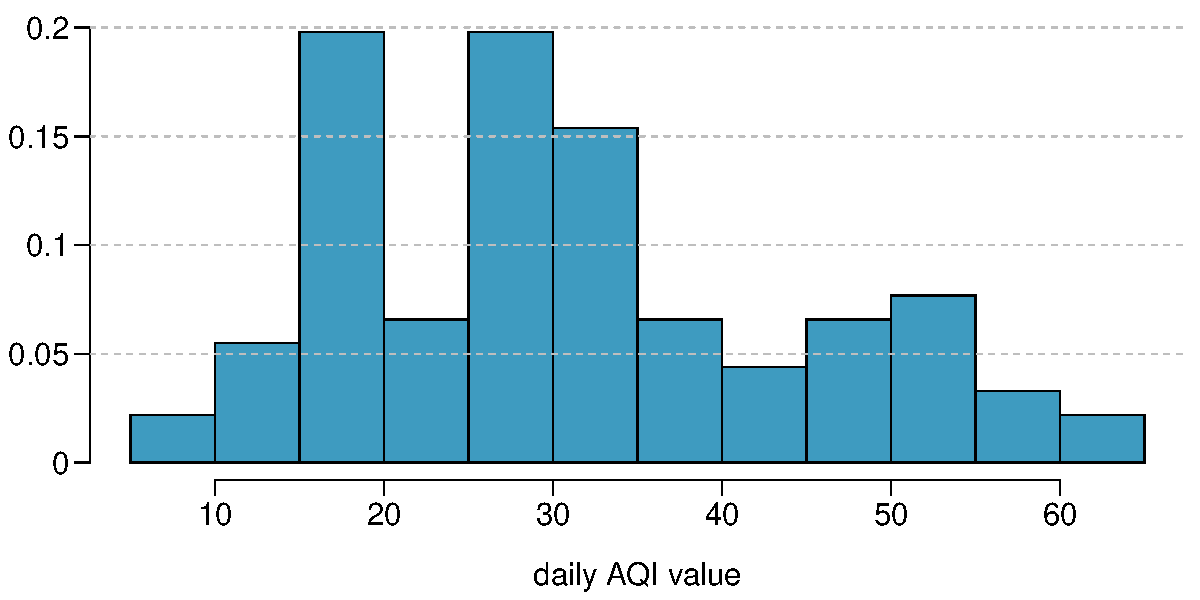
\includegraphics[width = 0.75\textwidth]{01/figures/eoce/durhamAQI/durhamAQI_hist} 
\end{center}
\begin{parts}
\item Estimate the median AQI value of this sample.
\item Would you expect the mean AQI value of this sample to be higher or lower than the median? Explain your reasoning.
\item Estimate Q1, Q3, and IQR for the distribution.
\end{parts}
}{}


% 39

\eoce{\qt{Histograms and box plots} Compare the two plots below. What characteristics of the distribution are apparent in the histogram and not in the box plot? What characteristics are apparent in the box plot but not in the histogram?
\begin{center}
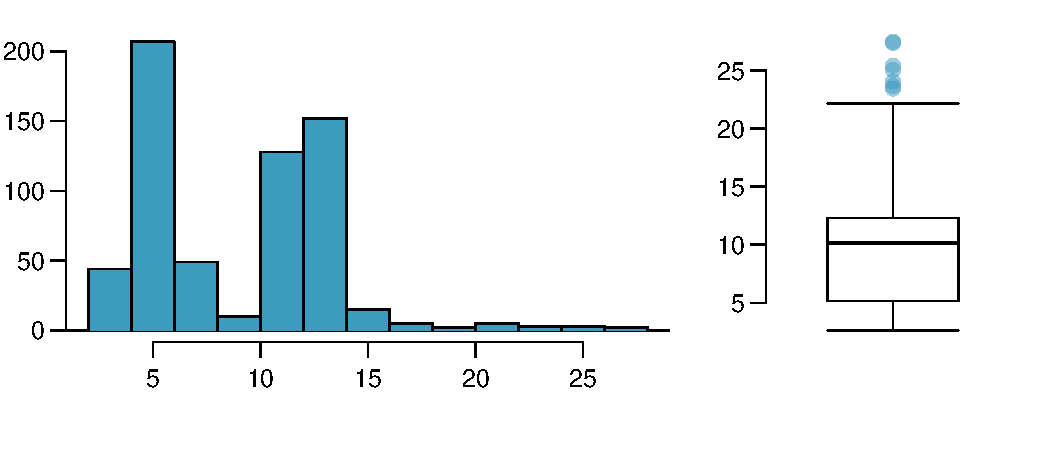
\includegraphics[width = 0.77\textwidth]{01/figures/eoce/bimodalHistBox/bimodalHistBox}
\end{center}
}{}


% 40
\textB{\pagebreak}

\eoce{\qt{Marathon winners\label{NYMarathon}} The histogram and box plots below show the distribution of finishing times for male and female winners of the New York Marathon between 1970 and 1999.
\begin{center}
\includegraphics[width=0.9\textwidth]{01/figures/eoce/marathon/marathon_histBox}
\end{center}
\begin{parts}
\item What features of the distribution are apparent in the histogram and not the box plot? What features are apparent in the box plot but not in the histogram?
\item What may be the reason for the bimodal distribution? Explain.
\item Compare the distribution of marathon times for men and women based on the box plot shown below.
\begin{center}
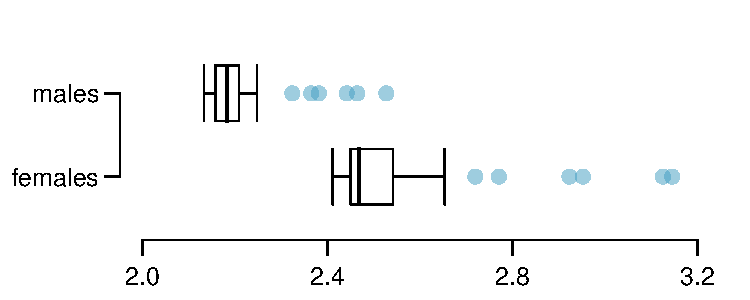
\includegraphics[width=0.7\textwidth]{01/figures/eoce/marathon/marathon_genderBox}
\end{center}
\item The time series plot shown below is another way to look at these data. Describe what is visible in this plot but not in the others.
\end{parts}
\begin{center}
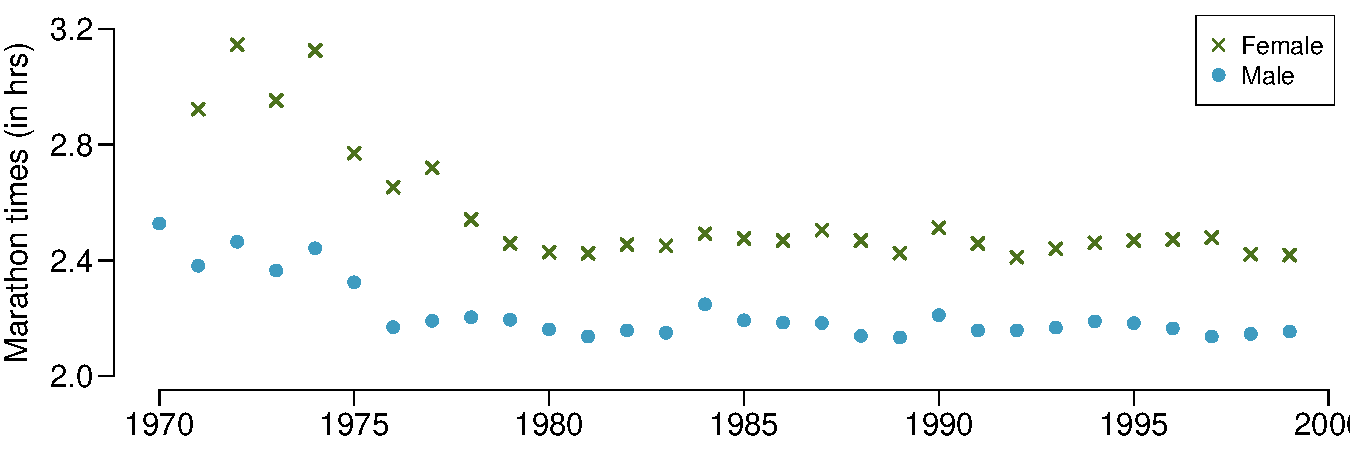
\includegraphics[width=0.95\textwidth]{01/figures/eoce/marathon/marathon_genderTimeSeries} \\
\end{center}
}{}


% 41
\textB{\pagebreak}

\eoce{\qt{Robust statistics} The first histogram below shows the distribution of the yearly incomes of 40 patrons at a college coffee shop. Suppose two new people walk into the coffee shop: one making \$225,000 and the other \$250,000. The second histogram shows the new income distribution. Summary statistics are also provided. \\
\begin{minipage}[c]{0.57\textwidth}
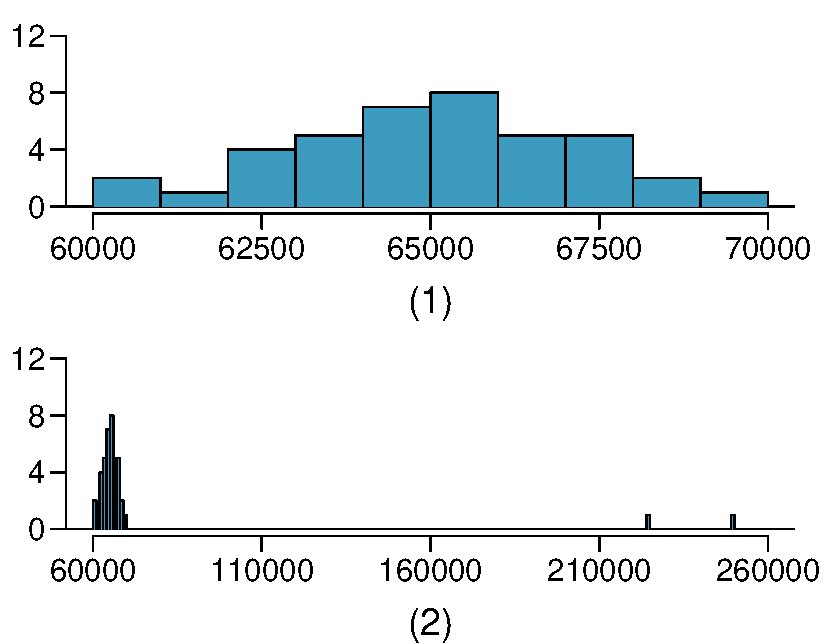
\includegraphics[width=\textwidth]{01/figures/eoce/salary/salary}
\end{minipage}
\begin{minipage}[c]{0.4\textwidth}
\begin{center}
\begin{tabular}{rrr}
  \hline
 & (1) & (2) \\ 
  \hline
n & 40 & 42 \\ 
  Min. & 60,680 & 60,680 \\ 
  1st Qu. & 63,620 & 63,710 \\ 
  Median & 65,240 & 65,350 \\ 
  Mean & 65,090 & 73,300 \\ 
  3rd Qu. & 66,160 & 66,540 \\ 
  Max. & 69,890 & 250,000 \\ 
  SD & 2,122 & 37,321 \\ 
   \hline
\end{tabular}
\end{center}
\end{minipage}
\begin{parts}
\item Would the mean or the median best represent what we might think of as a typical income for the 42 patrons at this coffee shop? What does this say about the robustness of the two measures?
\item Would the standard deviation or the IQR best represent the amount of variability in the incomes of the 42 patrons at this coffee shop? What does this say about the robustness of the two measures?
\end{parts}
}{}


% 42

\eoce{\qt{Distributions and appropriate statistics} For each of the following, describe whether you expect the distribution to be symmetric, right skewed, or left skewed. Also specify whether the mean or median would best represent a typical observation in the data, and whether the variability of observations would be best represented using the standard deviation or IQR.
\begin{parts}
\item Housing prices in a country where 25\% of the houses cost below \$350,000, 50\% of the houses cost below \$450,000, 75\% of the houses cost below \$1,000,000 and there are a meaningful number of houses that cost more than \$6,000,000.
\item Housing prices in a country where 25\% of the houses cost below \$300,000, 50\% of the houses cost below \$600,000, 75\% of the houses cost below \$900,000 and very few houses that cost more than \$1,200,000.
\item Number of alcoholic drinks consumed by college students in a given week.
\item Annual salaries of the employees at a Fortune 500 company.
\end{parts}
}{}


% 43

\noindent\begin{minipage}[c]{0.4\textwidth}
\eoce{\qt{Commuting times, Part I\label{workTravel}} The histogram to the right shows the distribution of mean commuting times in 3,143 US counties in 2010. Describe the distribution and comment on whether or not a log transformation may be advisable for these data.
}{} \vspace{5mm}
\end{minipage}%
\begin{minipage}[c]{0.58\textwidth}
\begin{center}
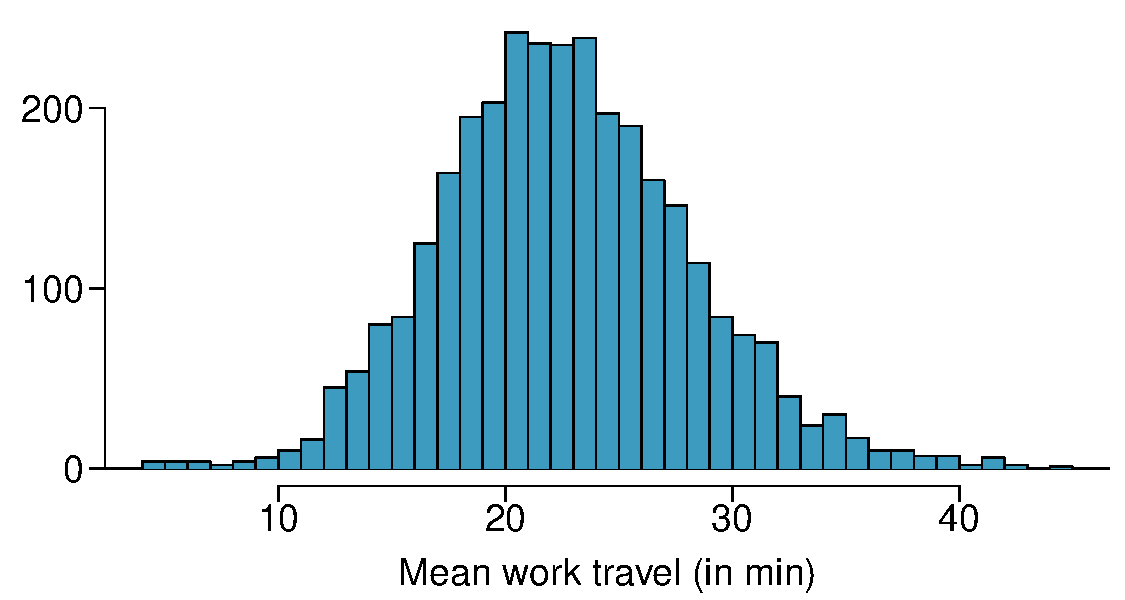
\includegraphics[width=\textwidth]{01/figures/eoce/county/county_workTravelHist}
\end{center}
\end{minipage}

\textB{\newpage}


% 44

\eoce{\qt{Hispanic population, Part I\label{hispHist}} The histogram below shows the distribution of the percentage of the population that is Hispanic in 3,143 counties in the US in 2010. Also shown is a histogram of logs of these values. Describe the distribution and comment on why we might want to use log-transformed values in analyzing or modeling these data.
\begin{center}
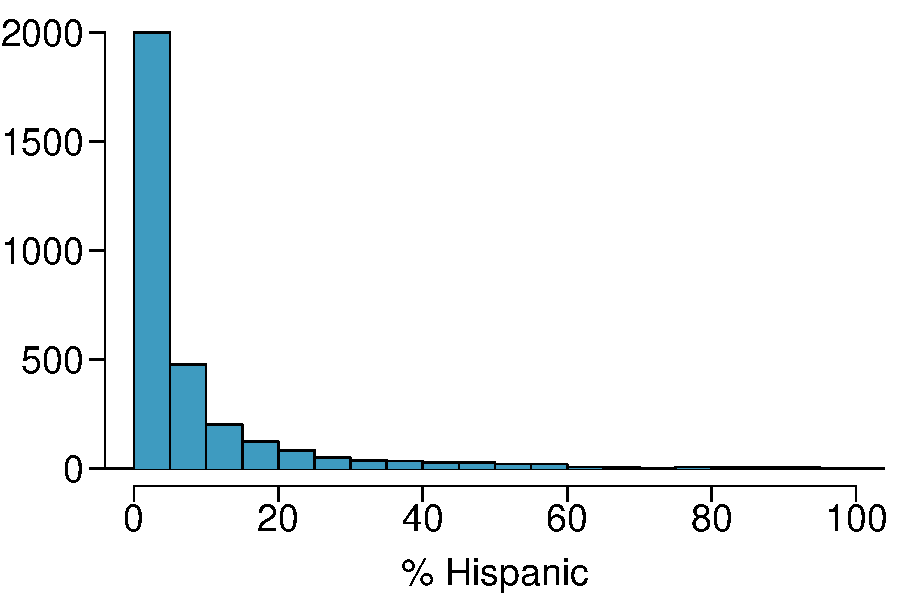
\includegraphics[width=0.49\textwidth]{01/figures/eoce/county/county_hispHist}
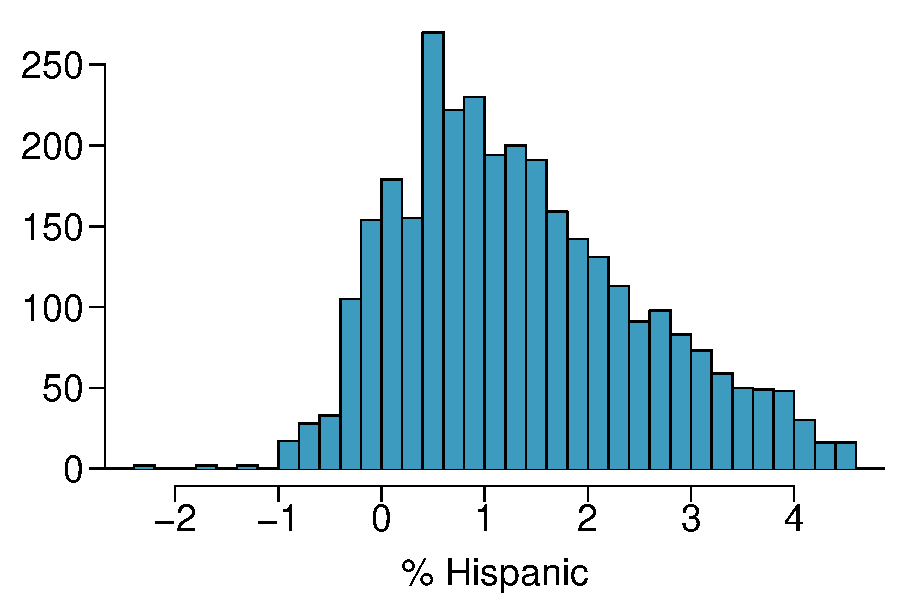
\includegraphics[width=0.49\textwidth]{01/figures/eoce/county/county_hispHistLog}
\end{center}
}{}



% 45

\eoce{\qt{Commuting times, Part II} Exercise~\ref{workTravel} displays histograms of mean commuting times in 3,143 US counties in 2010. Describe the spatial distribution of commuting times using the map below.
\begin{center}
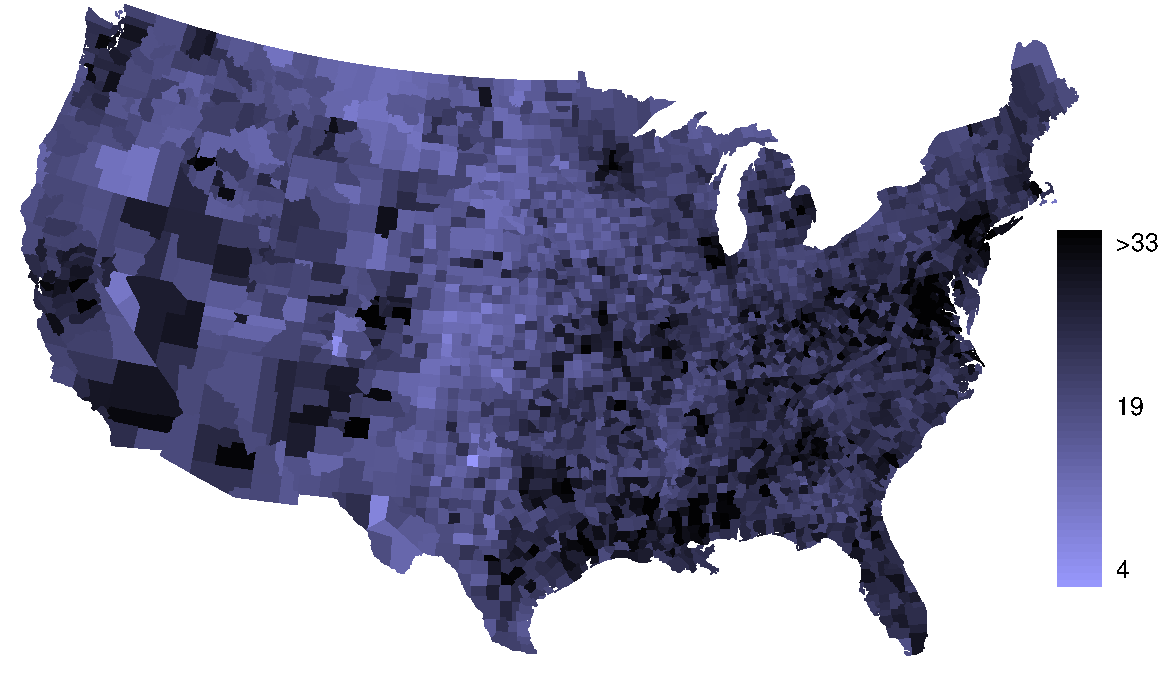
\includegraphics[width=\textwidth]{01/figures/eoce/county/county_workTravelMap}
\end{center}
}{}


% 46
\textB{\pagebreak}

\eoce{\qt{Hispanic population, Part II} Exercise~\ref{hispHist} displays histograms of the distribution of the percentage of the population that is Hispanic in 3,143 counties in the US in 2010.
\begin{center}
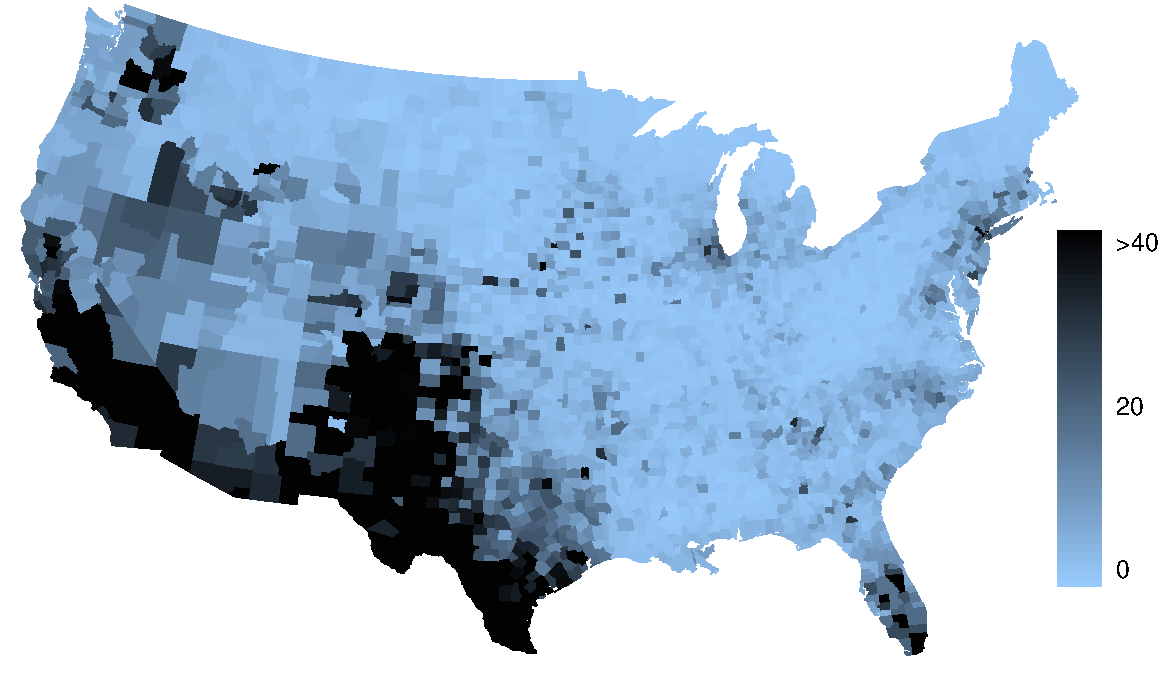
\includegraphics[width=\textwidth]{01/figures/eoce/county/county_hispMap}
\end{center}
\begin{parts}
\item What features of this distribution are apparent in the map but not in the histogram? 
\item What features are apparent in the histogram but not the map?
\item Is one visualization more appropriate or helpful than the other? Explain your reasoning.
\end{parts}
}{}


%_________________
\subsection{Considering categorical data}

% 47

\eoce{\qt{Antibiotic use in children} The bar plot and the pie chart below show the distribution of pre-existing medical conditions of children involved in a study on the optimal duration of antibiotic use in treatment of tracheitis, which is an upper respiratory infection.
\begin{parts}
\item What features are apparent in the bar plot but not in the pie chart?
\item What features are apparent in the pie chart but not in the bar plot?
\item Which graph would you prefer to use for displaying these categorical data?
\end{parts}
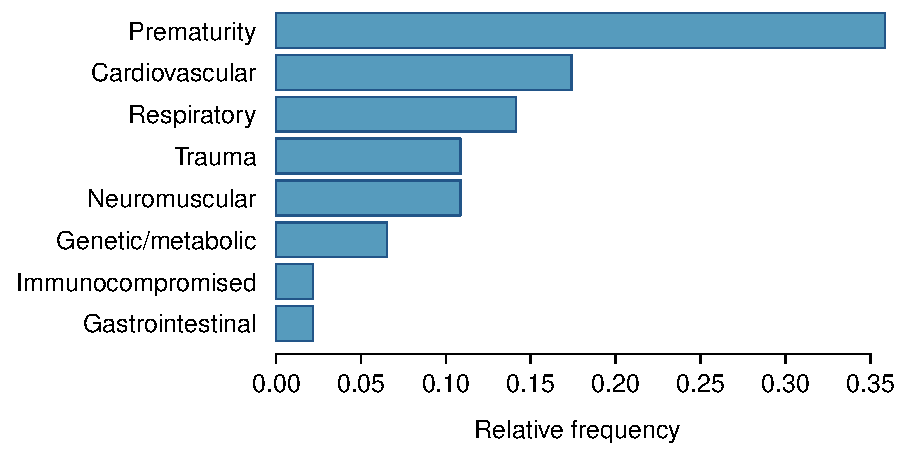
\includegraphics[width = 0.6\textwidth]{01/figures/eoce/tracheitis/tracheitis_bar}
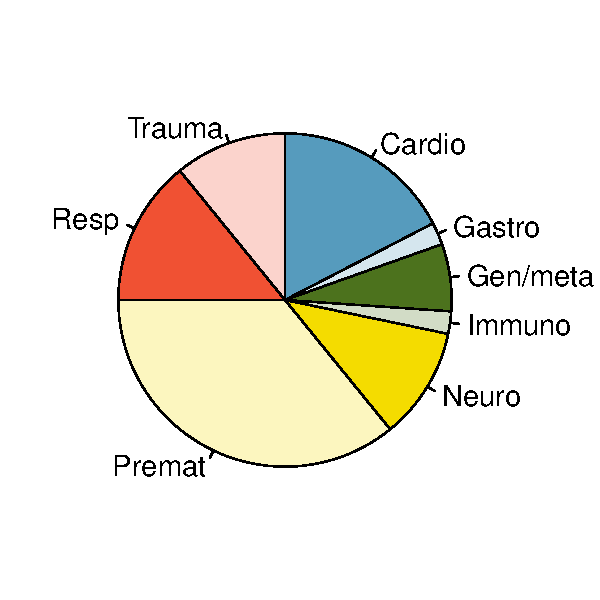
\includegraphics[width = 0.35\textwidth]{01/figures/eoce/tracheitis/tracheitis_pie}
}{}


% 48
\textB{\pagebreak}

\eoce{\qt{Views on immigration\label{immigration}} 910 randomly sampled registered voters from Tampa, FL were asked if they thought workers who have illegally entered the US should be (i) allowed to keep their jobs and apply for US citizenship, (ii) allowed to keep their jobs as temporary guest workers but not allowed to apply for US citizenship, or (iii) lose their jobs and have to leave the country. The results of the survey by political ideology are shown below.\footfullcite{survey:immigFL:2012}
\begin{center}
\begin{tabular}{l l  c c c c}
				&		& \multicolumn{3}{c}{\textit{Political ideology}} \\
\cline{3-5}
				& & Conservative	& Moderate	& Liberal 	& Total \\
\cline{2-6}
& (i) Apply for citizenship	& 57			& 120		& 101	& 278 \\
& (ii) Guest worker		& 121		& 113		& 28		& 262 \\
\raisebox{1.5ex}[0pt]{\emph{Response}} &(iii) Leave the country	& 179		& 126		& 45		& 350 \\ 
& (iv) Not sure			& 15			& 4			& 1		& 20\\
\cline{2-6}
& Total				& 372		& 363		& 175	& 910
\end{tabular}
\end{center}
\begin{parts}
\item What percent of these Tampa, FL voters identify themselves as conservatives?
\item What percent of these Tampa, FL voters are in favor of the citizenship option?
\item What percent of these Tampa, FL voters identify themselves as conservatives and are in favor of the citizenship option?
\item What percent of these Tampa, FL voters who identify themselves as conservatives are also in favor of the citizenship option? What percent of moderates and liberal share this view?
\item Do political ideology and views on immigration appear to be independent? Explain your reasoning.
\end{parts}
}{}


% 49

\noindent\begin{minipage}[c]{0.5\textwidth}
\eoce{\qt{Views on the DREAM Act} The same survey from Exercise~\ref{immigration} also asked respondents if they support the DREAM Act, a proposed law which would provide a path to citizenship for people brought illegally to the US as children. Based on the mosaic plot shown on the right, are views on the DREAM Act and political ideology independent?
}{}
\vspace{3mm}
\end{minipage}
\begin{minipage}[c]{0.5\textwidth}
\begin{center}
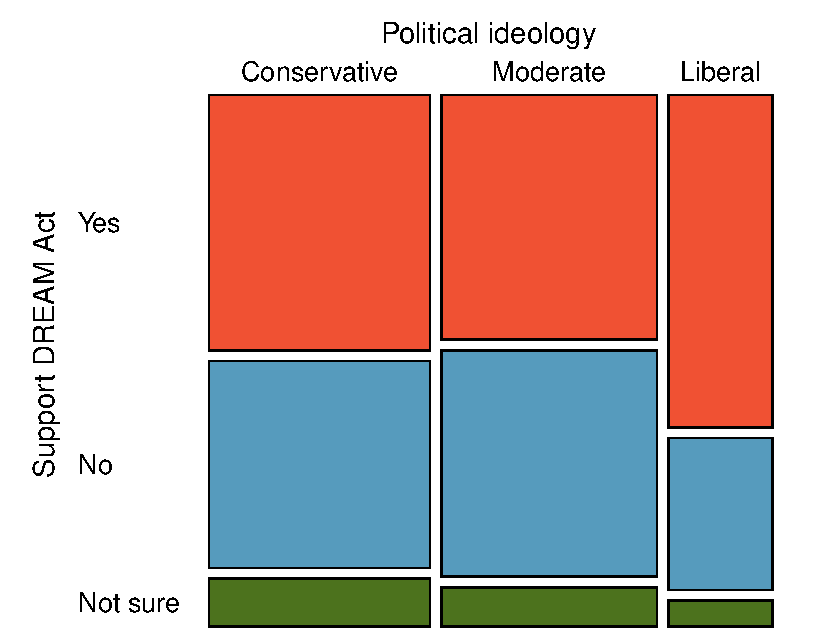
\includegraphics[width = 0.85\textwidth]{01/figures/eoce/dreamAct/dreamAct_mosaic}
\end{center}
\end{minipage} \vspace{3mm}

% 50

\eoce{\qt{Heart transplants, Part I\label{HeartTr}} The Stanford University Heart Transplant Study was conducted to determine whether an experimental heart transplant program increased lifespan. Each patient entering the program was designated an official heart transplant candidate, meaning that he was gravely ill and would most likely benefit from a new heart. Some patients got a transplant and some did not. The variable \texttt{transplant} indicates which group the patients were in; patients in the treatment group got a transplant and those in the control group did not. Another variable called \texttt{survived} was used to indicate whether or not the patient was alive at the end of the study. \textB{Figures may be found on the next page.} \footfullcite{Turnbull+Brown+Hu:1974}
\begin{parts}
\item Based on the mosaic plot, is survival independent of whether or not the patient got a transplant? Explain your reasoning.
\item What do the box plots suggest about the efficacy (effectiveness) of transplants?
\end{parts}
\begin{center}
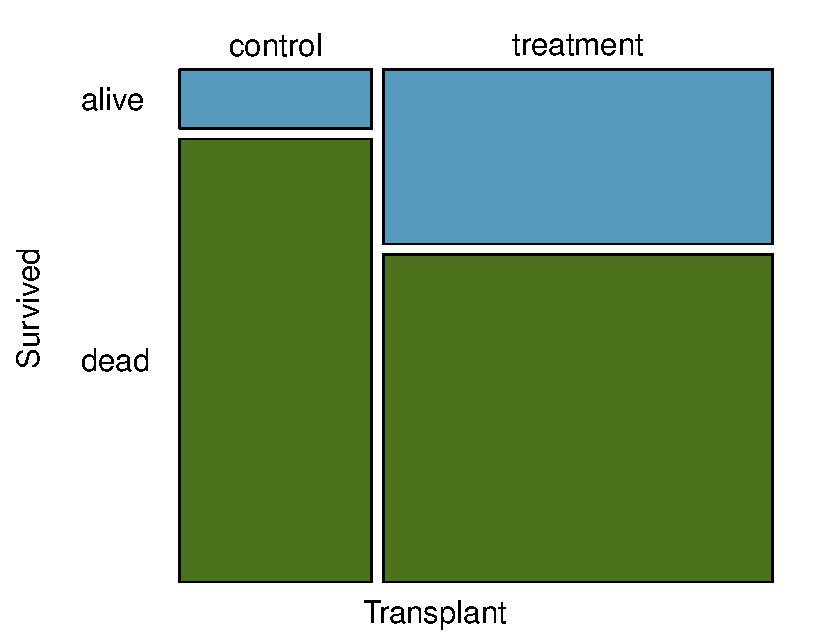
\includegraphics[width= 0.48\textwidth]{01/figures/eoce/heartTr/heartTr_SurvTrMosaic}\ 
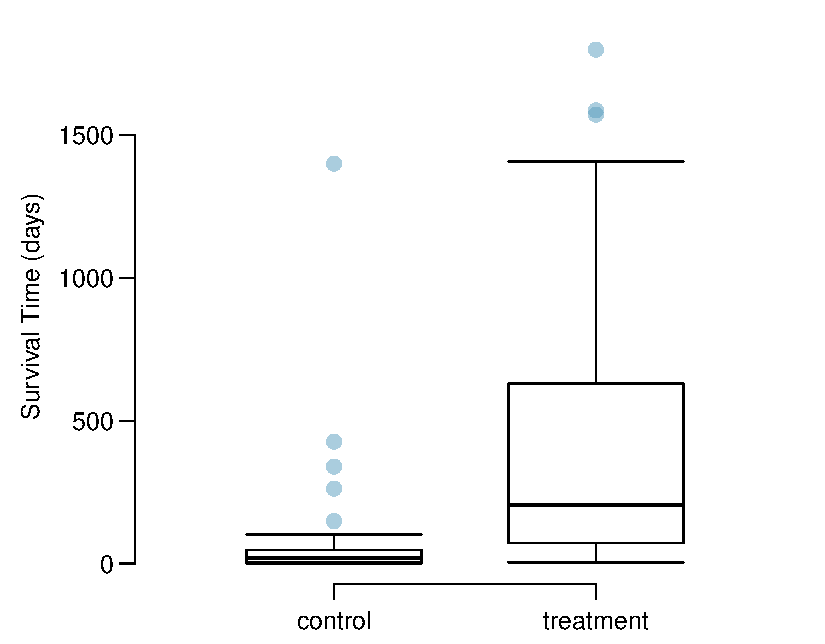
\includegraphics[width = 0.48\textwidth]{01/figures/eoce/heartTr/heartTr_SurvTimeTrBox}
\end{center}
}{}


%_________________
\subsection{Case study: gender discrimination}

% 51

\eoce{\qt{Side effects of Avandia, Part I\label{AvandiaTrueFalse}} Rosiglitazone is the active ingredient in the controversial type~2 diabetes medicine Avandia and has been linked to an increased risk of serious cardiovascular problems such as stroke, heart failure, and death. A common alternative treatment is pioglitazone, the active ingredient in a diabetes medicine called Actos. In a nationwide retrospective observational study of 227,571 Medicare beneficiaries aged  65 years or older, it was found that 2,593 of the 67,593 patients using rosiglitazone and 5,386 of the 159,978 using pioglitazone had serious cardiovascular problems. These data are summarized in the contingency table below. \footfullcite{Graham:2010}
\begin{center}
\begin{tabular}{ll  cc c} 
								&				& \multicolumn{2}{c}{\textit{Cardiovascular problems}} \\
\cline{3-4}	
								&				& Yes 	& No 		& Total	\\
\cline{2-5}
\multirow{2}{*}{\textit{Treatment}}		& Rosiglitazone 	& 2,593	& 65,000		& 67,593 	\\
								& Pioglitazone		& 5,386 	& 154,592 	& 159,978\\
\cline{2-5}
								&Total			& 7,979	& 219,592		& 227,571
\end{tabular}
\end{center}
Determine if each of the following statements is true or false. If false, explain why. \textit{Be careful:} The reasoning may be wrong even if the statement's conclusion is correct. In such cases, the statement should be considered false.
\begin{parts}
\item Since more patients on pioglitazone had cardiovascular problems (5,386 vs. 2,593), we can conclude that the rate of cardiovascular problems for those on a pioglitazone treatment is higher.
\item The data suggest that diabetic patients who are taking rosiglitazone are more likely to have cardiovascular problems since the rate of incidence was (2,593 / 67,593 = 0.038) 3.8\% for patients on this treatment, while it was only (5,386 / 159,978 = 0.034) 3.4\% for patients on pioglitazone.
\item The fact that the rate of incidence is higher for the rosiglitazone group proves that rosiglitazone causes serious cardiovascular problems.
\item Based on the information provided so far, we cannot tell if the difference between the rates of incidences is due to a relationship between the two variables or due to chance.
\end{parts}
}{}


% 52
\textB{\pagebreak}

\eoce{\qt{Heart transplants, Part II} Exercise~\ref{HeartTr} introduces the Stanford Heart Transplant Study. Of the 34 patients in the control group, 4 were alive at the end of the study. Of the 69 patients in the treatment group, 24 were alive. The contingency table below summarizes these results.
\begin{center}
\begin{tabular}{ll  cc c} 
							&		& \multicolumn{2}{c}{\textit{Group}} \\
\cline{3-4}
							&		& Control 	& Treatment 	& Total	\\
\cline{2-5}
							& Alive 	& 4	 	& 24			& 28 	\\
\raisebox{1.5ex}[0pt]{\emph{Outcome}} & Dead	& 30		& 45	 		& 75\\
\cline{2-5}
							& Total	& 34		& 69			& 103
\end{tabular}
\end{center}
\begin{parts}
\item What proportion of patients in the treatment group and what proportion of patients in the control group died?
\item One approach for investigating whether or not the treatment is effective is to use a randomization technique.
\begin{subparts}
\item What are the claims being tested?
\item  The paragraph below describes the set up for such approach, if we were to do it without using statistical software. Fill in the blanks with a number or phrase, whichever is appropriate.
\begin{adjustwidth}{2em}{2em}
We write \textit{alive} on \rule{2cm}{0.5pt} cards representing patients who were alive at the end of the study, and \textit{dead} on \rule{2cm}{0.5pt} cards representing patients who were not. Then, we shuffle these cards and split them into two groups: one group of size \rule{2cm}{0.5pt} representing treatment, and another group of size \rule{2cm}{0.5pt} representing control. We calculate the difference between the proportion of \textit{dead} cards in the treatment and control groups (treatment - control) and record this value. We repeat this many times to build a distribution centered at \rule{2cm}{0.5pt}. Lastly, we calculate the fraction of simulations where the simulated differences in proportions are \rule{2cm}{0.5pt}. If this fraction is low, we conclude that it is unlikely to have observed such an outcome by chance and that the null hypothesis (independence model) should be rejected in favor of the alternative.
\end{adjustwidth}
\item What do the simulation results shown below suggest about the effectiveness of the transplant program?
\end{subparts}
\end{parts}
\begin{center}
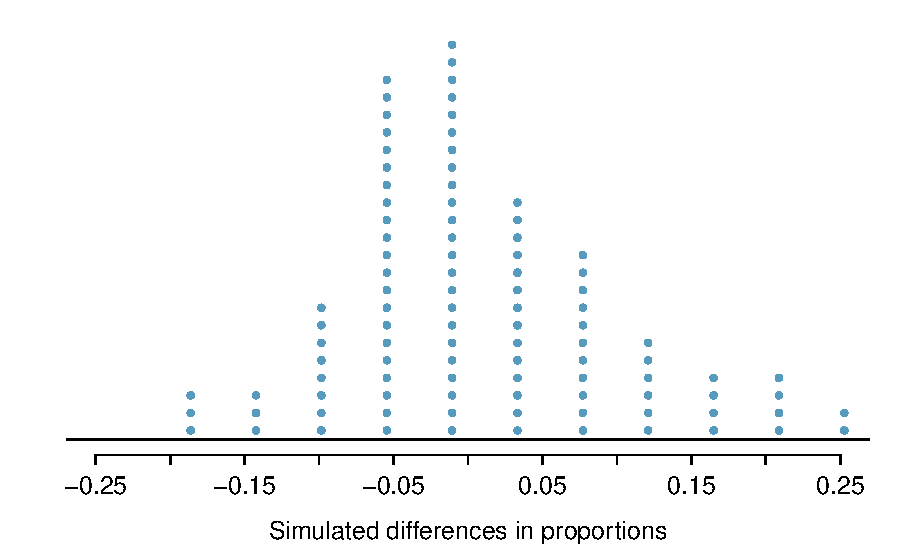
\includegraphics[width = 0.75\textwidth]{01/figures/eoce/heartTr/heartTr_RandHist} \\
\end{center}
}{}


% 53
\textB{\pagebreak}

\eoce{\qt{Side effects of Avandia, Part II} Exercise~\ref{AvandiaTrueFalse} introduces a study that compares the rates of serious cardiovascular problems for diabetic patients on rosiglitazone and pioglitazone treatments. The table below summarizes the results of the study.
\begin{center}
\begin{tabular}{ll  cc c} 
								&				& \multicolumn{2}{c}{\textit{Cardiovascular problems}} \\
\cline{3-4}	
								&				& Yes 	& No 		& Total	\\
\cline{2-5}
\multirow{2}{*}{\textit{Treatment}}		& Rosiglitazone 	& 2,593	& 65,000		& 67,593 	\\
								& Pioglitazone		& 5,386 	& 154,592 	& 159,978\\
\cline{2-5}
								&Total			& 7,979	& 219,592		& 227,571
\end{tabular}
\end{center}
\begin{parts}
\item What proportion of all patients had cardiovascular problems?
\item If the type of treatment and having cardiovascular problems were independent, about how many patients in the rosiglitazone group would we expect to have had cardiovascular problems?
\item We can investigate the relationship between outcome and treatment in this study using a randomization technique.  While in reality we would carry out the simulations required for randomization using statistical software, suppose we actually simulate using index cards. In order to simulate from the independence model, which states that the outcomes were independent of the treatment, we write whether or not each patient had a cardiovascular problem on cards, shuffled all the cards together, then deal them into two groups of size 67,593 and 159,978. We repeat this simulation 1,000 times and each time record the number of people in the rosiglitazone group who had cardiovascular problems. Below is a relative frequency histogram of these counts. \\
\begin{subparts}
\item What are the claims being tested?
\item Compared to the number calculated in part (b), which would provide more support for the alternative hypothesis,  \textit{more} or \textit{fewer} patients with cardiovascular problems in the rosiglitazone group?
\item What do the simulation results suggest about the relationship between taking rosiglitazone and having cardiovascular problems in diabetic patients?
\end{subparts}
\begin{center}
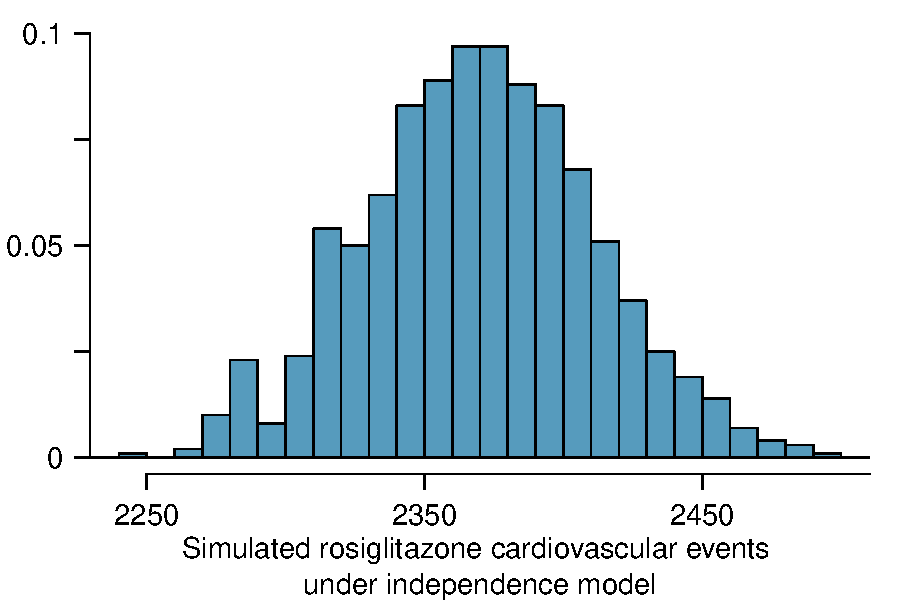
\includegraphics[width = 0.75\textwidth]{01/figures/eoce/avandia/avandia_RandHist} \\
\end{center}
\end{parts}
}{}


% 54
\textB{\pagebreak}

\eoce{\qt{Sinusitis and antibiotics, Part II} Researchers studying the effect of antibiotic treatment compared to symptomatic treatment for acute sinusitis randomly assigned 166 adults diagnosed with sinusitis into two groups (as discussed in Exercise~\ref{sinusitis}). Participants in the antibiotic group received a 10-day course of an antibiotic, and the rest received symptomatic treatments as a placebo. These pills had the same taste and packaging as the antibiotic. At the end of the 10-day period patients were asked if they experienced improvement in symptoms since the beginning of the study. The distribution of responses is summarized below. \footfullcite{Garbutt:2012}
\begin{center}
\begin{tabular}{ll  cc c} 
			&				& \multicolumn{2}{c}{\textit{Self reported}} \\
			&				& \multicolumn{2}{c}{\textit{improvement in symptoms}} \\
\cline{3-4}
			&							& Yes 	& No 	& Total	\\
\cline{2-5}
							&Antibiotic 	& 66	 	& 19		& 85 	\\
\raisebox{1.5ex}[0pt]{\textit{Treatment}}	& Placebo		& 65	 	& 16 	 	& 81 \\
\cline{2-5}
							&Total		& 131	& 35		& 166
\end{tabular}
\end{center}
\begin{parts}
\item What type of a study is this?
\item Does this study make use of blinding?
\item At first glance, does antibiotic or placebo appear to be more effective for the treatment of sinusitis? Explain your reasoning using appropriate statistics.
\item There are two competing claims that this study is used to compare: the independence model and the alternative model. Write out these competing claims in easy-to-understand language and in the context of the application. \textit{Hint:} The researchers are studying the effectiveness of antibiotic treatment.
\item Based on your finding in (c), does the evidence favor the alternative model? If not, then explain why. If so, what would you do to check if whether this is strong evidence?
\end{parts}
}{}
